
\documentclass[12pt]{article}

\usepackage{physor2016}

\usepackage{amsmath}
\usepackage{bm}
\usepackage{caption}
\usepackage{subcaption}

\newcommand{\yr}{2}
\newcommand{\ve}[1]{\ensuremath{\mathbf{#1}}}
\newcommand{\Macro}{\ensuremath{\Sigma}}
\newcommand{\vOmega}{\ensuremath{\hat{\Omega}}}
\newcommand{\omvec}{\ensuremath{\hat{\Omega}}}
\newcommand{\rvec}{\ensuremath{\vec{r}}}
\newcommand{\vecr}{\ensuremath{\vec{r}}}
\newcommand{\co}{CADIS-$\Omega$ }


\pagestyle{myheadings}

\usepackage{graphicx}
\usepackage{tikz}
\usepgflibrary{shapes.geometric}
\usepackage{hyperref}
\hypersetup{
    colorlinks,
    citecolor=black,
    filecolor=black,
    linkcolor=black,
    urlcolor=black
}

\usepackage{booktabs}

\usepackage{siunitx}
%------------------------------------------------------------------------------

%------------------------------------------------------------------------------
% Define title. Use all CAPITALS.
%------------------------------------------------------------------------------
\title{Improved Hybrid Modeling of Spent Fuel Storage Facilities}
%\subtitle{}
%
% ...and authors
%
\author{ 
  Year \yr Annual Report for Project 14-6378\\
  January 2016 to December 2016\\
  \\
  \\
  Prepared by:\\
  Rachel Slaybaugh (PI), Assistant Professor \\
  Department of Nuclear Engineering, University of California, Berkeley \\
  4173 Etcheverry Hall, Berkeley, CA 94720, USA\\
  +1 570 850 3385, 
  \href{mailto:slaybaugh@berkeley.edu}{slaybaugh@berkeley.edu}\\
  \\
 Co-Is: Thomas Evans, Scott Moser\\
  Oak Ridge National Laboratory\\
  \\
  \\
  Performed Under: NEUP Award DE-NE0008286\\
  Project period: 01/01/15 - 12/31/17 \\
  \\
  TPOC: Piyush Sabharwall\\
  FPOC: Daniel Vega\\
  \\
  \\
  Submitted March 31, 2017
}
  
%------------------------------------------------------------------------------
  

%------------------------------------------------------------------------------
% Setup PDF info. This sets several values which are listed as the "properties"
% of the PDF file.
%------------------------------------------------------------------------------
\hypersetup{
  pdftitle=\shorttitle,
  pdfauthor=\shortauthor
}


\begin{document}

%\doublespacing

%\linenumbers

%------------------------------------------------------------------------------
% Make the titlepage and set the pagestyle to fancy throughout
%------------------------------------------------------------------------------
\maketitle
\clearpage
\tableofcontents
\clearpage
%\begin{abstract}
%A new method for generating variance reduction parameters for strongly anisotropic, deep-penetration radiation shielding studies is presented. This method generates an alternate form of the adjoint scalar flux quantity, $\phi^{\dagger}_{\Omega}$, which is used by both CADIS and FW-CADIS to generate variance reduction parameters for local and global response functions, respectively. The new method, called CADIS-$\Omega$, was implemented in the Denovo/ADVANTG software suite, and results are presented for a concrete labyrinth test problem. Results indicate that the flux generated by CADIS-$\Omega$ incorporates localized angular anisotropies in the flux effectively. CADIS-$\Omega$ outperformed CADIS in the test problem while obtaining correct results. This initial work indicates that CADIS-$\Omega$ may be highly useful for shielding problems with strong angular anisotropies. A future test plan to fully characterize the new method is proposed, which should reveal more about the types of realistic problems for which the CADIS-$\Omega$ will be suited. 
%\end{abstract}
%
%\keywords{Hybrid Methods, CADIS, FW-CADIS, Angular Biasing}

%------------------------------------------------------------------------------
%
%------------------------------------------------------------------------------
%\section*{Executive Summary}
%\label{sect::summary}
%\clearpage

\section{Project Description}
\label{sect::project}

In this project, we are developing variance reduction methods for computational neutral particle transport intended to improve the ability to design and operate systems in which particle streaming is important, such as monitoring systems for interim used fuel installations. 
We are using Exnihilo \cite{evans_denovo:_2010}, MCNP \cite{brown_mcnp_2002}, and ADVANTG \cite{mosher_new_2010}, which will make our new tool widely available and easily usable. 
These innovative analysis tools will enable next generation nuclear material management for existing and future U.S.\ nuclear fuel cycles, minimizing proliferation and terrorism risk.

Storage casks are particularly challenging for radiation transport calculations because they are characterized by dense shields followed by streaming paths to the detectors. 
The impact of streaming is amplified in arrays of casks because detectors can only see rear casks through air paths between front casks. 
Deterministic methods suffer from ray effects between the casks and detectors, making solutions unreliable. 
Monte Carlo methods are challenged by getting particles out of the cask into the region of interest, and can therefore require unreasonably large calculation times to achieve acceptable statistical uncertainties in the computed tallies.

This report describes current technology in \autoref{sect::current} and the mathematics of our new method in \autoref{sect::omega}. This is followed by significant developments in \autoref{sect::sig-devel}, a comparison of our projected vs.\ actual performance in \autoref{sect::perf-comp}, and results and accomplishments in \autoref{sect::accomplishments}. This is followed by the cost and schedule status in \autoref{sect::cost} and \autoref{sect::schedule}, respectively; changes in \autoref{sect::changes}, anticipated issues in \autoref{sect::issues}, personnel changes in \autoref{sect::personnel}, and finally, products in \autoref{sect::products}.  

%------------------------------------
\subsection{Current Technology}
\label{sect::current}
Cutting-edge variance reduction methods that speed up Monte Carlo calculations often use deterministic solutions to make weight window maps. 
Perhaps the most widespread and accessible of these methods are the Consistent Adjoint Driven Importance Sampling (CADIS) \cite{wagner_automatic_1997,wagner_automated_1998,haghighat_monte_2003} and Forward-Weighted CADIS (FW-CADIS) \cite{wagner_forward-weighted_2007,wagner_forward-weighted_2009,wagner_forward-weighted_2010} methods. 
These methods create consistently-biased source distributions and weight window targets using a coarse determinstic solution for the adjoint scalar flux, $\phi^{\dagger}$, as a measure of the importance. 

In general, we are interested in finding some response, $R$, characterized by some response function $f(\ve{r}, E)$ in some volume $V_f$:
%
\begin{equation}
 R = \int_E \int_{V_f} f(\ve{r}, E) \phi(\ve{r}, E) dV dE \:,
 \label{eq:Response}
\end{equation}
where $\phi(\ve{r}, E)$ is the forward scalar flux, which describes how neutrons flow from the source $q(\ve{r}, E)$ to contribute to the response. 
Note that the adjoint scalar flux, $\phi^{\dagger}(\ve{r}, E)$, represents how each part of phase space contributes to the adjoint ``source" ($q^{\dagger}(\ve{r}, E)$, which can be set as the response of interest). 
Thus, $\phi^{\dagger}$ represents the expected contribution of a source particle to the desired response.
 
With this in mind, we can create variance reduction parameters for use in MC. 
We coarsely and quickly perform a deterministic calculation to get $\phi^{\dagger}(\ve{r}, E)$.
Equations \eqref{eq:CADISmethod} describe the biasing parameters generated by CADIS and FW-CADIS (jointly referred to as FW/CADIS). 
%
\begin{subequations} 
\label{eq:CADISmethod} 
\begin{equation}
\hat{q}(\vec {r} ,E)  = \frac{\phi^{\dagger}(\vec {r} ,E)q(\vec {r} ,E)}{\iint\phi^{\dagger}(\vec {r} ,E)q(\vec {r} ,E) dE d\vec{r}} \\
         = \frac{\phi^{\dagger}(\vec {r} ,E)q(\vec {r} ,E)}{R} \:,
\label{eq:weightedsource}
\end{equation}
\begin{equation}
w_0(\vec {r} ,E)  = \frac{q}{\hat{q}} \\
     = \frac{R}{\phi^{\dagger}(\vec {r} ,E)} \:,
\label{eq:startingweight}
\end{equation}
\begin{equation}
\hat{w}(\vec {r} ,E) = \frac{R}{\phi^{\dagger}(\vec {r} ,E)} \:,
\label{eq:WW}
\end{equation}
\end{subequations}
where $\hat{q}$ is the biased source distribution, $w_0$ is the starting weight of the particles, $\hat{w}$ is the target weight of the particles, and $R$ is the response of interest. 
For the standard implementations, these items are a function of space and energy only.

For problems with strong anisotropies in the particle flux, the importance map and biased source developed using the space/energy treatment above may not represent the real importance well enough to sufficiently improve performance in the Monte Carlo calculation. 
Note that because the \textit{scalar} adjoint flux is used in Eqns.~\eqref{eq:CADISmethod}, the angular dependence of the importance function is not retained. 
Thus, no information is retained on how particles move towards the response function. 
The drawback of this simplification is that, within a given space/energy cell, the map provides the average importance of a particle moving in \textit{any direction} through the cell\textemdash excluding information about how particles move \textit{toward} the objective. 
However, if the angular dependence of the importance function were fully retained, the map would be very large (tens or hundreds of GB) and more costly to use in the Monte Carlo simulation. 

An example of missing important angular behavior can be seen in this maze problem. 
A 10MeV isotropic point source is next to a concrete maze followed by an NaI detector. 
This problem has vacuum boundary conditions. 
In \autoref{fig:maze} one can see the geometry and forward flux. 
\autoref{fig:orig-adj} shows the adjoint flux. 
We can see that (a) this is representing how areas of phase space contribute to the solution and (b) that no angular information is being captured.
In a vacuum system, particles that exit the back of the geometry should not affect the detector. 
This behavior is being missed by the standard method, and thus not speeding up MC as well as it could. 
\begin{figure}
\centering
\begin{subfigure}{.75\textwidth}
  \centering
  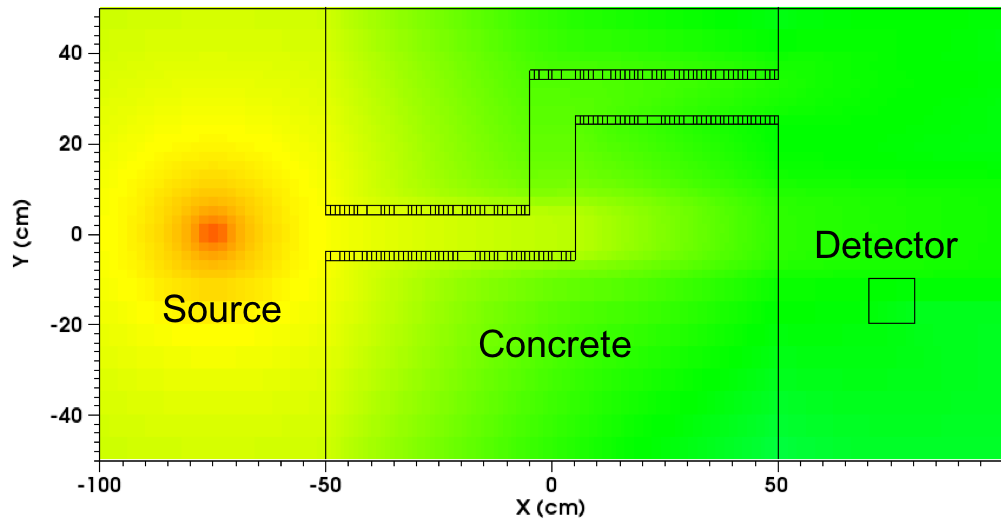
\includegraphics[height=2in,clip]{maze-forward.png}
  \caption{Forward Flux}
  \label{fig:maze}
\end{subfigure}%
\begin{subfigure}{.25\textwidth}
  \centering
  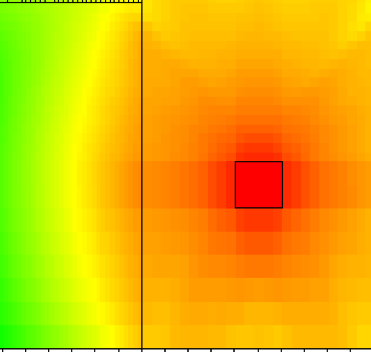
\includegraphics[height=1.1in,clip]{maze-adj-orig.png}
  \caption{Adjoint Close Up}
  \label{fig:orig-adj}
\end{subfigure}
\caption{Concrete Maze with 10 MeV isotropic point source and NaI detector}
\label{fig:adjoint}
\end{figure}

Interim used fuel installations exhibit strong angular anisotropies, and therefore the ability to simulate them effectively for nuclear material management is limited with current tools. 
This led us to develop a new method, which we're calling the FW/CADIS-$\Omega$ method. 
In MC without performance improvement, relative error (Re) decreases as the square of time (t). 
Thus, we measure improving a calculation by using the Figure of Merit (FOM):
\begin{equation}
\text{FOM}=\frac{1}{Re^{2}t}\:.
\end{equation}?

%---------------------------------
\subsection{CADIS-$\Omega$}
\label{sect::omega}
To do fast, accurate transport for used fuel monitoring, we need an importance map generated quickly using deterministic methods that captures the impact of angle in the importance information. 
In this work we build on past methods, but calculate the adjoint scalar flux in a way that has not been done before.

Our new automated hybrid method, which we're calling FW/CADIS-$\Omega$, incorporates angular information into the biasing parameters for FW/CADIS while not explicitly biasing in angle. 
That is, we generate space- and energy-dependent importance maps that incorporate the flux anisotropy in a more effective way than current implementations without adding the complication of angular weight windows. 
FW/CADIS-$\Omega$ uses Eqns.~\eqref{eq:CADISmethod}, but generates the adjoint scalar flux differently. 

We use the idea of the contributon flux, defined in Eqn.~\eqref{eq.Cont-Flux}, in generating the adjoint scalar flux. 
Contributons are pseudo-particles that carry ``response" from the radiation source to a detector ~\cite{williams_generalized_1991,williams_contributorn_1992,williams_contributon_study}. 
%
\begin{equation}
\Psi (\vec {r},\:\hat\Omega ,E) = \psi^{\dagger} (\vec {r},\:\hat\Omega ,E) \psi(\vec {r} ,\:\hat\Omega,E)
\label{eq.Cont-Flux} 
\end{equation}
%
The contributon flux includes both forward and adjoint information, expressing the importance of a particle that is born at a forward source and moves through space towards an adjoint source, contributing to the solution.
An importance map made using contributon flux will assign high importance to particles that are created at the forward source and are likely to generate a response in the detector. 

In FW/CADIS-$\Omega$, we integrate the contributon flux over angle and divide by the integrated forward angular flux as shown in Eqn.~\eqref{eq:angularhybrid}.
This quantity, which we designate $\phi^{\dagger}_{\Omega}$, is then used in Eqns.~\eqref{eq:CADISmethod}, just like the standard FW/CADIS methods.
%
\begin{equation} 
\phi^{\dagger}_{\Omega}(\vec{r},E) = \frac{\int_{4\pi} \psi(\vec {r} ,E,\hat{\Omega})\psi^{\dagger}(\vec {r} ,E,\hat{\Omega})d\hat\Omega }{\int_{4\pi}\psi(\vec {r} ,E,\hat{\Omega})d\hat\Omega}
\label{eq:angularhybrid}
\end{equation}

In a strongly anisotropic system, the adjoint scalar flux generated by Eqn.~\eqref{eq:angularhybrid} will be influenced by which directions were most prominent in the forward case. 
We can see this by considering the contributon flux, the numerator of Eqn.~\eqref{eq:angularhybrid}.
Particles in $\phi^{\dagger}_{\Omega}$ include the impact of how the direction they are moving influences the answer, which should allow for more effective Monte Carlo transport when angular effects are important. 
Note that in an isotropic system, $\phi^{\dagger}_{\Omega}$ will be essentially the same as $\phi^{\dagger}$. 

We can see the impact of this newly-defined adjoint flux by looking at the maze problem from \autoref{fig:adjoint}.
\autoref{fig:new-adj} shows a close up of the adjoint flux from our new method.
In this case it is clear that particles going out the back of the problem are not expected to contribute to the detector. This is the kind of result that makes sense, and demonstrates the appropriate incorporation of angular information.
Furthermore, we see in \autoref{fig:maze-re} that this is reflected in CADIS-$\Omega$ obtaining a lower relative error than either CADIS or analog MC for the same number of particles.
Finally, \co obtained a FOM of 145, while CADIS's was only 5.1. 
This illustrates the type of improvement this project can achieve. 
\begin{figure}
\centering
\begin{subfigure}{.25\textwidth}
  \centering
  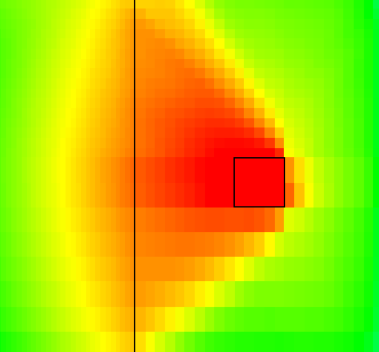
\includegraphics[height=1.1in,clip]{maze-adj-new.png}
  \caption{New Method Adjoint Close Up}
  \label{fig:new-adj}
\end{subfigure}%
\begin{subfigure}{.75\textwidth}
  \centering
  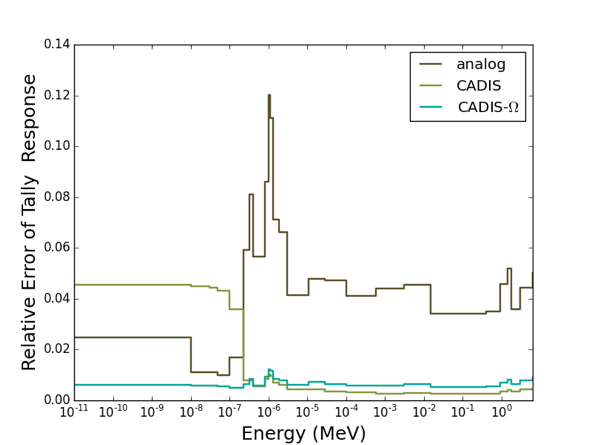
\includegraphics[height=3in,clip]{maze-re.png}
  \caption{Relative Error for Analog, CADIS, and CADIS-$\Omega$}
  \label{fig:maze-re}
\end{subfigure}
\caption{Concrete Maze Comparison}
\label{fig:adjoint}
\end{figure}



% ---------------------------------------------------
\section{Significant Developments}
\label{sect::sig-devel}

As of December 31, 2016, there have been several big developments that have a significant favorable impact on the project. 
Note that the UC Berkeley personnel working on this project are PI Rachel Slaybaugh, doctoral candidate Madicken Munk, first year student Marissa Ramirez-Zweiger, and research scientist Richard Vasques. 
We are being supported by Tom Evans, Tara Pandya, Seth Johnson, and Scott Mosher at Oak Ridge National Laboratory (ORNL). 
\begin{enumerate}
\item Code implementation is complete\\
Exnihilo, the deterministic code supplying adjoint flux values for weight windows, has been successfully modified to store and write adjoint flux (previously the only output was scalar flux). 
Further, an integration utility that implements Eqn.~\eqref{eq:angularhybrid} is also complete. 
Finally, we have automated the interface between the integration utility and ADVANTG, which will allow the full method to be used seamlessly using only ADVANTG input files. 

\item Software testing and documentation is complete\\
To ensure that the software is both correct and usable, we have tested the software--implementing unit tests where appropriate--and documented how to use the software. 
We have compared results from our new method with results we know to be correct. 
Further, we have developed scripts to automate the execution of our test problems as well as plotting and analysis of the results. 
Those scripts are available at this github repository: \url{https://github.com/munkm/thesiscode}. 
 
\item Method characterization is fully underway \\
We have a collection of small problems that incorporate anisotropy in different ways and to different degrees to investigate the new method's performance. 
Last year at this time we were not able to start calculations with the \co method. 
Thus, we had run some analog and CADIS calculations only.
Now, we have run all of our test problems with each method. 
We are in the process of fine tuning: sorting out which problems we need to run with more particles, which ones we want to investigate more fully, etc.

Further, we have developed a collection of metrics to characterize anisotropy. 
Each metric can be used to help us characterize how our method preforms for what types of problems:
\vspace*{-.5em}
      \begin{itemize}
      \item Scalar Contributon Ratio: If the adjoint or forward angular flux is significantly peaked in $\vOmega$, this will result in a deviation between the numerator and denominator because there will be a multiplicative effect in the angular flux captured in $\Phi_{c}$ and not $\phi_{c}$.
      \[M_{1} = \frac{\phi^{\dagger}(\vecr,E)\phi(\vecr,E)}{\int_{\vOmega}\psi^{\dagger}(\vecr,\vOmega,E)\psi(\vecr,\vOmega,E)} = \frac{\phi_{c}}{\Phi_{c}}\]
      
      \item Adjoint Flux Ratio: metric for comparing which regions have significantly differing bias parameters in standard-adjoint and omega-adjoint situations. This metric will deviate from unity if the forward flux is anisotropic.
      \[M_{2} = \frac{\phi^{\dagger}_{\vOmega}(\vecr,E)}{\phi^{\dagger}(\vecr,E)}\]
      
      \item Maximum to Average Flux Ratios: the ratio between the maximum and average angular contributon flux in each space-energy voxel. The higher this quantity, the more peaked the contributon flux is in $\Omega$. 
      \begin{align*}
      \psi^{c} &= \psi^{\dagger}(\vecr,E, \vOmega)\psi(\vecr,E, \vOmega)\\
      M_{3} &= \frac{\psi^c_{\max}}{\psi^{c}_{\text{avg}}}\\
      M_{4} &=  \frac{\frac{\psi^{c}_{\max}}{\psi^{c}_{\text{avg}}}}{\frac{\psi^{\dagger}_{\max}}{\psi^{\dagger}_{\text{avg}}}} 
      \end{align*} 
      
       \item Maximum to Minimum Flux Ratios: this quantity incorporates information about the behavior of the local maximum relative to the local minimum angular flux in each cell. This metric may be more appropriate to describe the anisotropy of the flux in cells where the distribution of flux values are not well reflected by the average flux.
       \begin{align*}
      M_{5} &= \frac{\psi^c_{\max}}{\psi^{c}_{\min}}\\
      M_{4} &=  \frac{\frac{\psi^{c}_{\max}}{\psi^{c}_{\min}}}{\frac{\psi^{\dagger}_{\max}}{\psi^{\dagger}_{\min}}}
       \end{align*}
      \end{itemize} 

 
\item A large, representative test problem input specification is complete\\
The main item of interest is how this work will effect storage cask simulation. 
We have a full spent fuel storage cask model with overpack constructed in the input format required for ADVANTG. 
We started with a SCALE cask model and added an overpack, including rebar. 
This model was contributed back to ORNL's cask modeling library. 
Next, this model was converted to MCNP input syntax for use with ADVANTG.
We've started running calculations with this model.
\end{enumerate}


% ---------------------------------------------------
\section{Performance Comparison}
\label{sect::perf-comp} 
%A written comparison of the actual project accomplishments with the project goals and objectives established for the reporting period; if goals and/or objectives for the reporting period were not met, a detailed description of the variance shall be provided. 
Project performance has lagged behind schedule in some areas from a timeline perspective.
This section will discuss the causes as well as correcting steps that have been taken.
Milestones for the project are given in \autoref{tab:milestones}.
\begin{table}[h!]
\begin{center}
\caption{Project Milestone Status as of Year \yr}
\begin{tabular}{ | l | l | l | l | }
\hline
\textbf{Level} & \textbf{Title} & \textbf{Proposed Completion} & \textbf{Actual Completion} \\ \hline
M2 & Year 1 Annual Report for Project 14-6378 & 4/1/16 & 4/11/16 \\
M2 & Year 2 Annual Report for Project 14-6378 & 4/1/17 & 4/1/17 \\ 
M2 & Final Report for Project 14-6378 & 3/31/18 & -- \\ \hline
M2 & Code & 9/30/16 & 11/15/16 \\
M3 & Background Research & 6/30/15 & 1/26/16 \\
M3 & Test and Document & 9/30/16 & 10/31/16 \\
M3 & Implementation & 9/30/16 & 10/31/16 \\  \hline
M2 & Testing & 12/31/16 & 12/31/16 \\
M3 & Baseline calculations & 12/31/16 & 11/30/16 \\
M3 & New method calculations & 9/30/16 & 11/30/16 \\ \hline
M2 & Angular sensitivity investigation & 1/31/17 & -- \\ \hline
M2 & Impact studies & 3/31/18 & -- \\
\hline
\end{tabular}
\label{tab:milestones}
\end{center}
\end{table}

Under the \textit{M2 Code} milestone, background research, testing and documentation, and implementation, began on schedule and are now completed. 
However, these items were all completed behind schedule. 
The main challenge in this area was the difficulty of building the Exnihilo software stack on certain compute architectures. 
We had originally planned to use Savio \cite{savio}, a condo-model cluster at UC Berkeley. 
However, Savio uses Intel compilers while Exnihilo really needs gnu compilers. 
As a result, we lost about three months of time--causing us to be late on implementation and testing and documentation (which had previously been ahead of schedule).
Ultimately, we abandoned the pursuit of using Savio and chose to build the software on computers at ORNL.
These delays have had a negative timeline impact on the entire project. 

The background research was reported as late because of the nature of background research. 
Ms.\ Munk, the primary student working on this, had completed background research before doing much code work.
However, because she would need to look up new things as implementation progressed, we realized it was not technically ``complete''.
At the beginning of the year the need to conduct more background research abated. 
This change in deadline did not impact project performance, but reflects the reality of continued information gathering.

We have completed the \textit{M2 Testing} work very close to on schedule. 
Inputs for all test problems are created, and initial runs completed (both baseline and new). 
Note that the new method calculations were delayed for the same reason that implementation was delayed.
We were unable to use the code before we had completed implementation. 

We have started the \textit{M2 Angular Sensitivity Investigation}, but this will also be completed behind schedule. 
This delay is in part from the implementation delay. 
We have also realized that many of the initial calculations did not use enough particles, so many problems need to be re-run for better results.
Finally, we paused this work when we realized we needed a better way of quantifying method performance. 
The development of the anisotropy metrics discussed in the \autoref{sect::sig-devel} section will enable us to do this.
Thus, we are much better setup to be able to appropriately quantify the angular sensitivity and method performance. 

We anticipate that the \textit{M2 Impact Studies} will be completed on time. 
As mentioned, we already received the cask model and updated it for use in calculations. 
Creating the input flies was several months worth of work, so having that completed already positions us very well for potentially being able to do more testing than originally planned. 


Last year the \textit{M2 Year 1 Annual Report} was submitted about two weeks late.  
The Principle Investigator (PI) failed to record that an Annual report was required and, as a result, did not begin the report until after the due date. 
The PI is now clearly aware of the need for the timely submission of the \textit{Year 2 Annual Report} budgeted time accordingly.
The PI will take the same actions for the Final report


% ---------------------------------------------------
\section{Accomplishments}
\label{sect::accomplishments}
%A discussion of what was accomplished under these goals and objectives established for this reporting period, including major activities, significant results, major findings or conclusions, key outcomes or other achievements.  This section should not contain any proprietary data or other information not subject to public release.  If such information is important to reporting progress, do not include the information, but include a note in the report advising the reader contact the Principal Investigator for further information. 

The main accomplishments have been nearing completion of code implementation and completion of the MCNP cask model. Full details of the model, including references and process for model development, are all recorded in this github repository: \url{https://github.com/munkm/caskmodels}. This record ensures provenance of the model, detailing the development, assumptions, construction process, barriers encountered, and final model. 

While not directly related to the project, Ms.\ Munk passed her PhD qualifying exam, the last major hurdle at UC Berkeley before the dissertation. This concrete personnel accomplishment forwards a side benefit of the project: training and development of the workforce. 


% ---------------------------------------------------
\section{Cost Status}
\label{sect::cost}
%Cost Status.  A comparison of the approved budget by budget period and the actual costs incurred during the reporting period shall be provided.  If cost sharing is required, the cost breakdown shall show the DOE share, recipient share, and total costs. 

Table~\ref{tab:costs} gives the proposed and actual project costs. The first column indicates the project item. The second two columns are the budgeted cost per item and total cost, respectively. The final two columns are the actual cost per item and total costs. Table~\ref{tab:differences} indicates the cost difference by item. 

\begin{table}[h!]
\begin{center}
\caption{Proposed and Actual Costs for Year \yr}
\begin{tabular}{ | l | l | l | l | l | }
\hline
	\textbf{Item} & \textbf{Per} & \textbf{Total} & \textbf{Actual} & \textbf{Total}\\ \hline
	\textit{Section A, Senior/Key Person} & &  \$12,429.33  &  &  \$18,883.07  \  \\ \hline
	\textit{Section B, Other Personnel} & &  \$94,058.52  &  &  \$94,254.35 \  \\ \hline
	\hspace*{1 em}Total Number Other Personnel & 4 & & \ 4 & \    \\ \hline
	\textit{Total Salary, Wages and Fringe Benefits (A+B)} & & \$106,487.85  &  &  \$113,137.42 \  \\ \hline
	\textit{Section C, Equipment} &  &  \$-    & \ &  \$-     \\ \hline
	\textit{Section D, Travel} & &  \$8,000 & & \$6,531.63   \\ \hline
	\hspace*{1 em}1.  Domestic & \$8,000 & &  \$6,531.63 & \  \\ \hline
	\hspace*{1 em}2.  Foreign &  \$-  & \   &  \$-    & \   \\ \hline
	\textit{Section E, Participant/Trainee Support Costs} & \ &  \$-    & \  &  \$-       \\ \hline
	\hspace*{1 em}1.  Tuition/Fees/Health Insurance &   \$-  & \   &  \$-      \ & \\ \hline
	\hspace*{1 em}2.  Stipends &  \$-   & \ &  \$-    & \    \\ \hline
	\hspace*{1 em}3.  Travel &  \$-    & \ &  \$-    & \   \\ \hline
	\hspace*{1 em}4.  Subsistence &  \$-    & \ &  \$-     & \  \\ \hline
	\hspace*{1 em}5.  Other &  \$-    & \  &  \$-    & \  \\ \hline
	\hspace*{1 em}6.  Number of Participants/Trainees & 0 & \ & 0 & \   \\ \hline
	\textit{Section F, Other Direct Costs}& \ & \$42,228.00  &  &  \$746.59     \\ \hline
	\hspace*{1 em}1.  Materials and Supplies & \$1,728.00  &  &  \$746.59  & \  \\ \hline
	\hspace*{1 em}2.  Publication Costs & \$500  &  &  \$-   & \  \\ \hline
	\hspace*{1 em}3.  Consultant Services &  \$-    & \ &  \$-     & \  \\ \hline
	\hspace*{1 em}4.  ADP/Computer Services &  \$-    & \  &  \$-    & \  \\ \hline
	\hspace*{1 em}5.  Subawards/Consortium/Contractual Costs &  \$- & \   &  \$-      & \  \\ \hline
	\hspace*{1 em}6.  Equipment or Facility Rental/User Fees &  \$-   & \  &  \$-     & \  \\ \hline
	\hspace*{1 em}7.  Alterations and Renovations &  \$-  & \  &  \$-      & \  \\ \hline
	\hspace*{1 em}8.  Computer laptops (2) & \$-  & & \$-  & \  \\ \hline
	\hspace*{1 em}9. Oak Ridge National Laboratory &  \$40,000 &  &  \$40,000    & \  \\ \hline
	\hspace*{1 em}10. Other 3 &  \$-    & \ &  \$-      & \  \\ \hline
	\textit{Section G, Direct Costs (A thru F)} &  &\$156,716  &  &  \$160,416  \  \\ \hline
	\textit{Section H, Indirect Costs} &  & \$- & & \$54,858 \  \\ \hline
	\textit{Section I, Total and Indirect Costs (G + H)} & &  \$212,959  &  &  \$215,274 \  \\ \hline
	\textit{Section J, Fee} & \ &  \$-   & \ &  \$-       \\ \hline
\end{tabular}
\label{tab:costs}
\end{center}
\end{table}

\begin{table}[h!]
\begin{center}
\caption{Cost Differences Year \yr}
\begin{tabular}{ | l | l | l | }
\hline
	\textbf{Item} & \textbf{Diff Per} & \textbf{Diff Total} \\ \hline
	\textit{Section A, Senior/Key Person} &  & \$(6,453.74) \\ \hline
	\textit{Section B, Other Personnel} &  & \$(195.83)  \\ \hline
	\hspace*{1 em}Total Number Other Personnel &  & \  \\ \hline
	\textit{Total Salary, Wages and Fringe Benefits (A+B)} &  & \$(6,649.57)  \\ \hline
	\textit{Section C, Equipment} &  &  \$-    \\ \hline
	\textit{Section D, Travel} &  & \$1,468.37 \\ \hline
	\hspace*{1 em}1.  Domestic & \$1,468.37 & \  \\ \hline
	\hspace*{1 em}2.  Foreign &  \$-    & \  \\ \hline
	\textit{Section E, Participant/Trainee Support Costs} & \ &  \$-      \\ \hline
	\hspace*{1 em}1.  Tuition/Fees/Health Insurance &  \$-    & \  \\ \hline
	\hspace*{1 em}2.  Stipends &  \$-    & \  \\ \hline
	\hspace*{1 em}3.  Travel &  \$-    & \  \\ \hline
	\hspace*{1 em}4.  Subsistence &  \$-    & \  \\ \hline
	\hspace*{1 em}5.  Other &  \$-    & \  \\ \hline
	\hspace*{1 em}6.  Number of Participants/Trainees &  \$-    & \  \\ \hline
	\textit{Section F, Other Direct Costs} &  & \$1,481.41 \\ \hline
	\hspace*{1 em}1.  Materials and Supplies & \$981.41 & \  \\ \hline
	\hspace*{1 em}2.  Publication Costs & \$500 & \  \\ \hline
	\hspace*{1 em}3.  Consultant Services &  \$-    & \  \\ \hline
	\hspace*{1 em}4.  ADP/Computer Services &  \$-    & \  \\ \hline
	\hspace*{1 em}5.  Subawards/Consortium/Contractual Costs &  \$-    & \  \\ \hline
	\hspace*{1 em}6.  Equipment or Facility Rental/User Fees &  \$-    & \  \\ \hline
	\hspace*{1 em}7.  Alterations and Renovations &  \$-    & \  \\ \hline
	\hspace*{1 em}8.  Computer laptops (2) & \$- & \  \\ \hline
	\hspace*{1 em}9. Oak Ridge National Laboratory &  \$-    & \  \\ \hline
	\hspace*{1 em}10. Other 3 &  \$-    & \  \\ \hline
	\textit{Section G, Direct Costs (A thru F)} &  & \$(3,699.79) \\ \hline
	\textit{Section H, Indirect Costs} &  & \$(54,857.89) \\ \hline
	\textit{Section I, Total and Indirect Costs (G + H)} &  & \$(2,314.72) \\ \hline
	\textit{Section J, Fee }&  &  \$-    \\ \hline
\end{tabular}
\label{tab:differences}
\end{center}
\end{table}

We are currently \$42,171.50 underspent compared to the budget (positive values in Table~\ref{tab:differences} are amount underspent). 
The primary reason for underspending is the length of time it took to identify an appropriate project researcher. 
Dr.\ Richard Vasques was hired in September 2015 and works part time on this project.
He will continue to be partially supported on this project throughout year 2, which we expect to align predicted spending with budgeted spending. 


% ---------------------------------------------------
\section{Schedule Status}
\label{sect::schedule}
%Schedule Status.  List milestones, anticipated completion dates and actual completion dates.  If you submitted a project management plan with your application, you must use this plan to report schedule and budget variances.   

As discussed in Section~\ref{sect::accomplishments}, the project is on schedule and we anticipate making future milestone deadlines.


% ---------------------------------------------------
\section{Changes}
\label{sect::changes}
%Describe any changes during the reporting period in project approach and the reasons for these changes.  Remember, significant changes to the project objectives and scope require prior approval by the Contracting Officer. 

The main change to the project scope is that we no longer plan to implement our method in MAVRIC~\cite{peplow_mavric_2011}, which is part of the SCALE package~\cite{SCALE}, and will only implement in ADVANTG. Originally, we had planned to use both because implementing in one is not much more difficult than implementing in another. However, we have since realized that outside of ORNL people are using ADVANTG more frequently than MAVRIC. Further, Douglas Peplow, the lead MAVRIC developer, has changed roles at ORNL and is no longer on this project. For these reasons the additional work to include MAVRIC is (a) larger than when we started and (b) unlikely to be worth it. We are therefore only focusing on ADVANTG. We anticipate the impact of this change to be negligible.


% ---------------------------------------------------
\section{Anticipated Issues}
\label{sect::issues}
%Describe any actual or anticipated problems or delays and any actions taken or plan to resolve them.

We had some initial delay in getting personnel in place at Berkeley, but that is resolved. We do not anticipate further problems or delays in that regard.

The largest problem we have encountered has been in building the software on the local cluster at Berkeley. The Exnihilo-ADVANTG system is fairly complex, requiring many software support packages. The software developers use gnu compilers (e.g.\ gcc), but the cluster at Berkeley, called Savio, uses Intel compilers. This has caused a very long delay while we work with the Savio team to resolve all of the software issues. We are still coming up with a long term solution that will be rapid and easy to use.


% ---------------------------------------------------
\section{Personnel Changes}
\label{sect::personnel}
%Describe any absence or changes of key personnel or changes in consortium/teaming arrangements during the reporting period. 

Douglas Peplow changed roles inside of ORNL and is no longer part the project. Dr.\ Peplow was in charge of the MAVRIC integration piece, which we have now cut from the project. We have been working with John Scaglione and Josh Jarrell to coordinate our cask models. Finally, Seth Johnson and Tara Pandya (all at ORNL) are now interfacing with UCB about Exnihilo-ADVANTG integration.


% ---------------------------------------------------
\section{Products}
\label{sect::products}
%List and describe any product produced or technology transfer activities accomplished during this reporting period, such as: \\
%a)	Publications (list journal name, volume, issue); conference papers; or other public releases of results.  Attach or send copies of the public releases to the DOE Program Manager. \\
%Publications: PHYSOR 2016 paper, ``FW/CADIS-$\Omega$: AN ANGLE-INFORMED HYBRID METHOD FOR DEEP-PENETRATION RADIATION TRANSPORT" can be found here\\ \url{http://munkm.github.io/papers/munk\_physor16.pdf}
%b)	Web site or other Internet sites (list the URL) that reflect the results of this project. \\
\textit{Website:} Our primary product through December 2015 has been our GitHub website: \\\href{https://github.com/munkm/caskmodels}{https://github.com/munkm/caskmodels}. This contains code use information, brainstorming, publicly-available details about the cask, process development, and citations. 

%c)	Networks or collaborations fostered. \\
\textit{Networks or collaborations:} We have grown the collaboration between ORNL and UCB, with Ms.\ Munk spending a few months at ORNL learning the codes and building our network.
%d)	Technologies/Techniques (identify and describe each). \\

\textit{Technologies or Techniques:} As described in the proposal, the new method is our main technology being developed. 
%e)	Inventions/Patent Applications (identify and describe with date of application) \\

%f)	Other products, such as data or databases, physical collections, audio or video, software or NetWare, models, educational aid or curricula, instruments or equipment (identify and describe).
\textit{Other products:} The full cask model we developed is a valuable ``other product", which has been contributed back to ORNL for use by the wider community.







\bibliographystyle{physor2016}
\bibliography{year1-annual-report}

\appendix

\makeatletter
\def\@seccntformat#1{APPENDIX \csname the#1\endcsname.~}
\makeatother

%------------------------------------------------------------------------------
% If you need to make one (or more) appendix (appendices), place them here as
% sections
%%------------------------------------------------------------------------------
%\section{HOW TO MAKE APPENDICES}
%\label{app::a}
%
%This is a placeholder for my first appendix
%
%\section{OTHER APPENDIX STUFF}
%\label{app::b}
%
%This is a placeholder for my second appendix

\end{document}

